Som en del af manageren skal der være en indstillings side til at aktivere eller deaktivere moduler. Dette afsnit beskriver denne side.

%guidelines
For at få en velkendt og standardiseret brugergrænseflade fulgtes Android design guidelines.
Disse guidelines angiver hvornår man skal bruger diverse knapper, actionbars, settings etc.
\citep{androiddesign}

%Prototypes
Ved at følge disse guidelines blev en række prototyper for indstillinger lavet.
Disse byggede på samme princip om at udarbejde en indstillingsmenu.
Der var diskussion om hvordan disse skulle være, men over flere iterationer valgtes der at gå fra en ``wizard'' tilgang til en regulær settings menu.
Dette skyldtes at indstillingssiden er tilpas simpel til en regulær settings menu og hvor en ``wizard'' tilgang ville forårsage unødig kompleksitet.
Billeder af diverse prototyper kan ses i \cref{fig:prototype-manager}

\begin{figure}[!h]
	\centering
	\begin{subfigure}[b]{0.45\textwidth}
			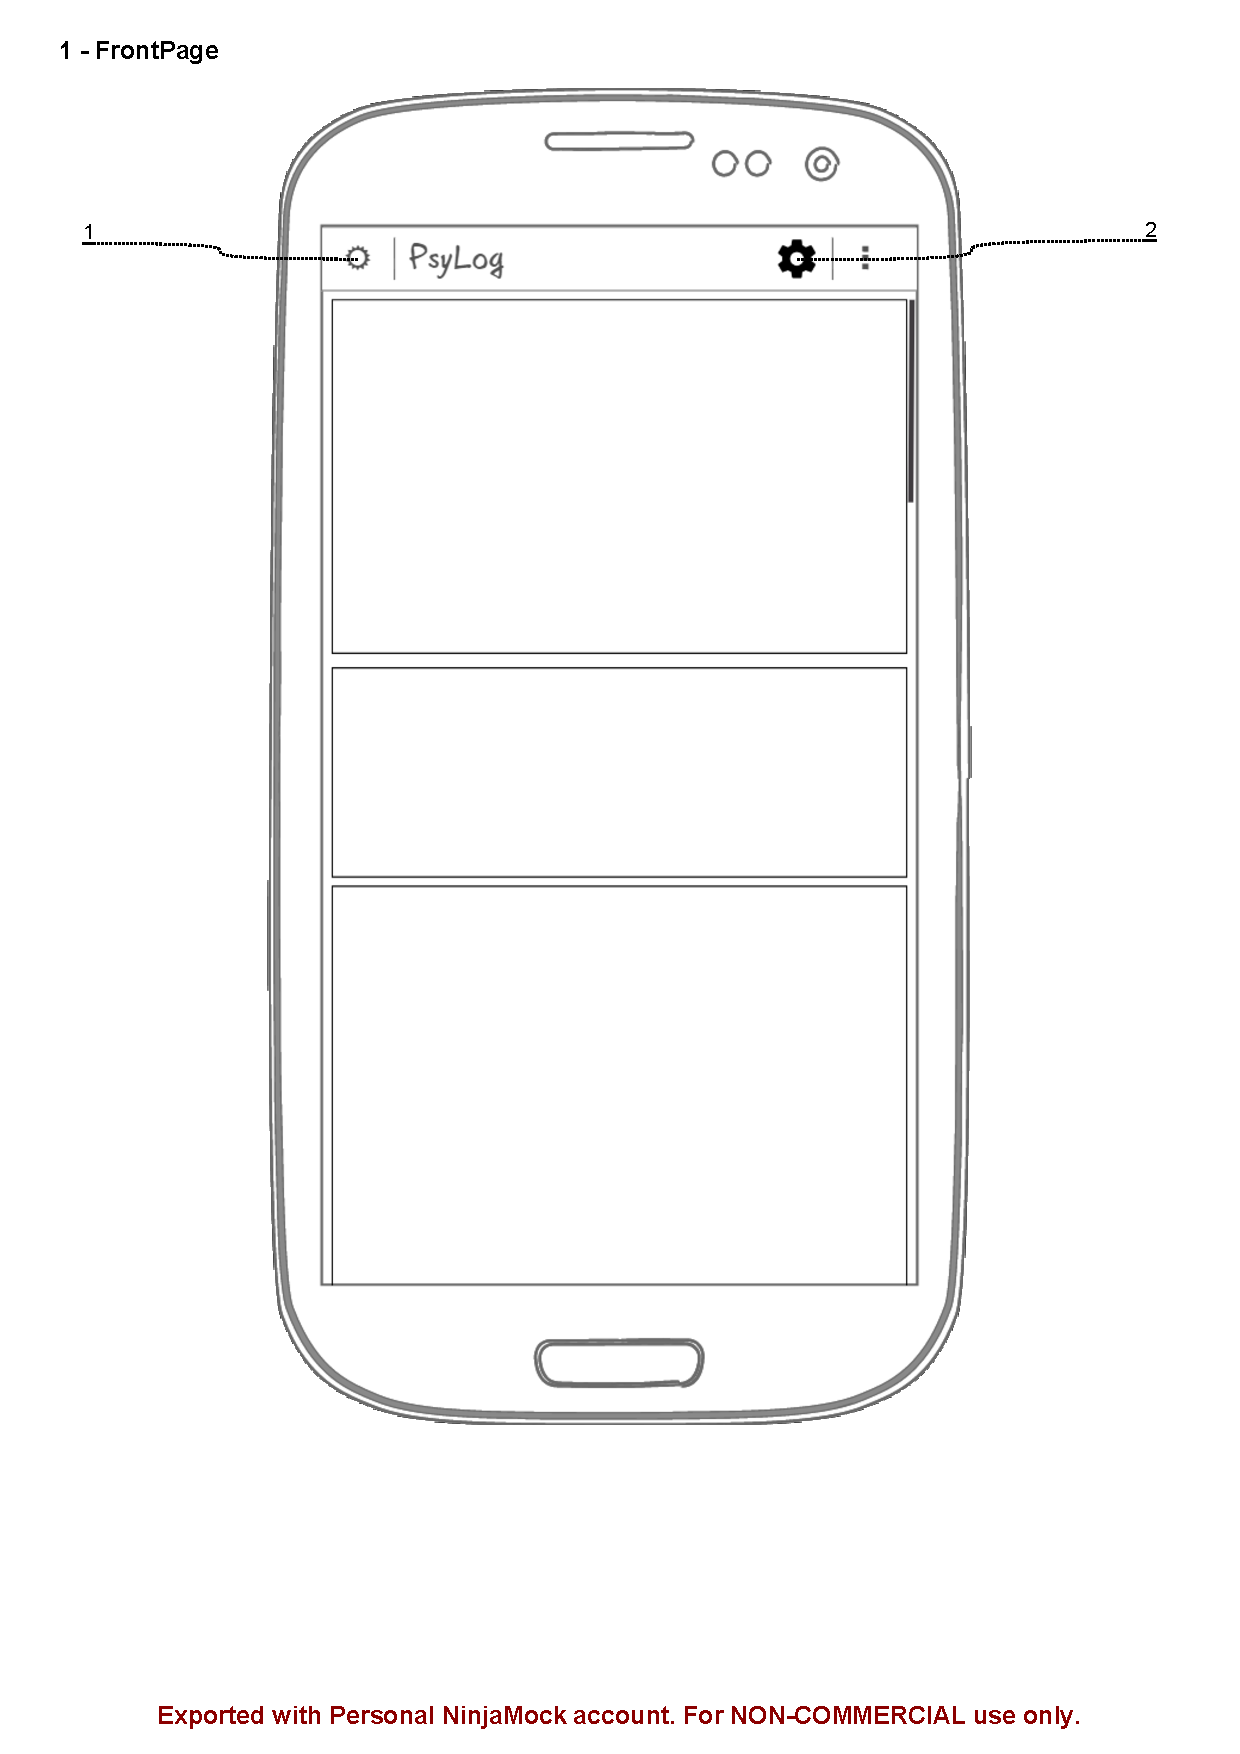
\includegraphics[scale=0.3, page=1, trim = 1cm 5.5cm 1cm 0cm, clip]{prototype.pdf}
			\caption{Forside}
	\end{subfigure}
	\begin{subfigure}[b]{0.45\textwidth}
			\includegraphics[scale=0.3, page=2, trim = 1cm 5.5cm 1cm 0cm, clip]{prototype.pdf}
			\caption{Indstillinger}
	\end{subfigure}
	\caption{Prototype af Manager}
	\label{fig:prototype-manager}
\end{figure}


%Actionbar
Ud fra prototypen kan man se en actionbar.
Tanken her er at følge et standard design hvor man har en actionbar i toppen.
Denne muliggør navigation til indstillinger, men også at gå tilbage til hovedmenuen.
Grunden til at dette er lavet er for at gøre det nemmere for brugeren at navigere rundt i selve programmet, hvis der f.eks. er mange undermenuer og man gerne vil tilbage til overmenuen.

%Indstillinger, checkbox
Til at angive om et givent modul skal være aktiveret eller ej bruges checkboxes.
Dette skyldes at det er et simpelt ja/nej valg. 
Tanken er at de moduler man har valgt, er dem der kører på smartphonen.

%indstillinger, dependencies og events
For at scanne mobilen for de moduler der er installeret bruges JSONParser der bliver beskrevet herunder.
Dette giver udslag i en række moduler der har afhængigheder af andre moduler.
JSONParseren giver som resultat en liste af moduler. Disse scannes så igennem for at finde deres afhængigheder.
Disse afhængigheder bruges så til at konstruere events til at fortælle de moduler der skal have besked når et givent modul aktiveres eller deaktiveres.
Ved at lave en sådan række er der implicit konstrueret en dependency graph.
Resultatet af dette er et slags hierarki hvor et modul på det lavest liggende niveau medfører en kæde af deaktiveringer af moduler der eksplicit og implicit afhænger af dette modul.
